% arara: lualatex
% arara: bib2gls
% arara: lualatex
% arara: lualatex
\documentclass[toc=listof]{scrreport}

\usepackage{fontspec}
\setmainfont{Linux Libertine O}

\usepackage{lipsum}

\usepackage
 [
   novref,
%   debug=showwrgloss
 ]{texjavahelp}

\hypersetup{colorlinks,linkcolor=blue}

\title{Test Document}
\author{Ann Author}

\GlsXtrLoadResources[src={\jobname},
 \TeXJavaHelpSymbolResourceOptions
]

\GlsXtrLoadResources[src={\jobname},
 \TeXJavaHelpGlsResourceOptions
]

\graphicspath{{images/}{images2/}}

\begin{document}
\maketitle

\frontmatter
\tableofcontents

\mainmatter
\chapter{Introduction}
\label{intro}

Reference \sectionref{sample}.
This is a \gls{test} document. 
A command starts with a \gls{bksl}.
\lipsum

\chapter{Sample}
\label{sample}

Reference \sectionref{intro}.
Reference \figureref{fig.sample}.

\FloatFig
{fig.sample}
{
\includegraphics[alt={Example Image}]{navbuttons}}
{Example Image}

\section{Sample Section}
\label{samplesection}

Reference \figureref{fig.sample-a}.

\FloatFig
{fig.sample-a}
{
\includegraphics[alt={Example Image A}]{secondaryNavButtons}}
{Example Image A}

\subsection{Sample Sub-Section}
\label{samplesubsection}

Reference \figureref{fig.sample-b}.

\FloatFig
{fig.sample-b}
{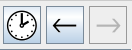
\includegraphics[alt={Example Image B}]{historybuttons}}
{Example Image B}


\printindex
\end{document}
